\chapter{Metodología}

\label{Chapter3}

En este capítulo se detallarán los procesos abordados para la extracción y clasificación de los dígitos escritos en los
telegramas de las elecciones. Primero se describirá el proceso de obtención, limpieza y transformación de los datos a
fin de obtener un dataset con el cual entrenar. Luego, se describirán los procesos a ser llevados a cabo para el diseño
experimental de los modelos.

\section{Descripción de los datos}

Los telegramas fueron descargados desde la \href{https://op.elecciones.gob.ar/telegramas/generales2021/}{página oficial
    del estado argentino}. Presentan un formato estándar en forma de grilla donde en cada renglón se encuentra el partido
político y los votos obtenidos para diputados y senadores. En la página también se puede descargar un CSV donde se
encuentra el {\it id} de cada telegrama y los valores digitalizados oficialmente.

\section{Extracción de dígitos de los telegramas}

Los telegramas de las elecciones de Santa Fe presentan un formato tabular, donde cada fila representa un partido
político y los votos obtenidos abiertos por senadores y diputados. Se debieron ejecutar múltiples pasos de extracción,
transformación y carga (ETL por sus siglas) de los mismos antes de poder armar un dataset con el cual entrenar los
modelos. Se utilizó la librería OpenCV \parencite{opencv_library} para manipular las imágenes y poder llevar a cabo el proceso de ETL.

\subsection{Enderezado}
Como los telegramas son escaneados a mano, el primer paso consiste en enderezarlos. Este proceso puede realizarse
buscando el rectángulo de mayor área, calculando el ángulo de rotación y rotando la imagen completa con la función
\verb|getRotationMatrix2D| de OpenCV.

\begin{figure}[H]
    \centering

    \tikzset{every picture/.style={line width=0.75pt}}

    \begin{tikzpicture}[x=0.75pt,y=0.75pt,yscale=-1,xscale=1]

        \draw (370,140) node  {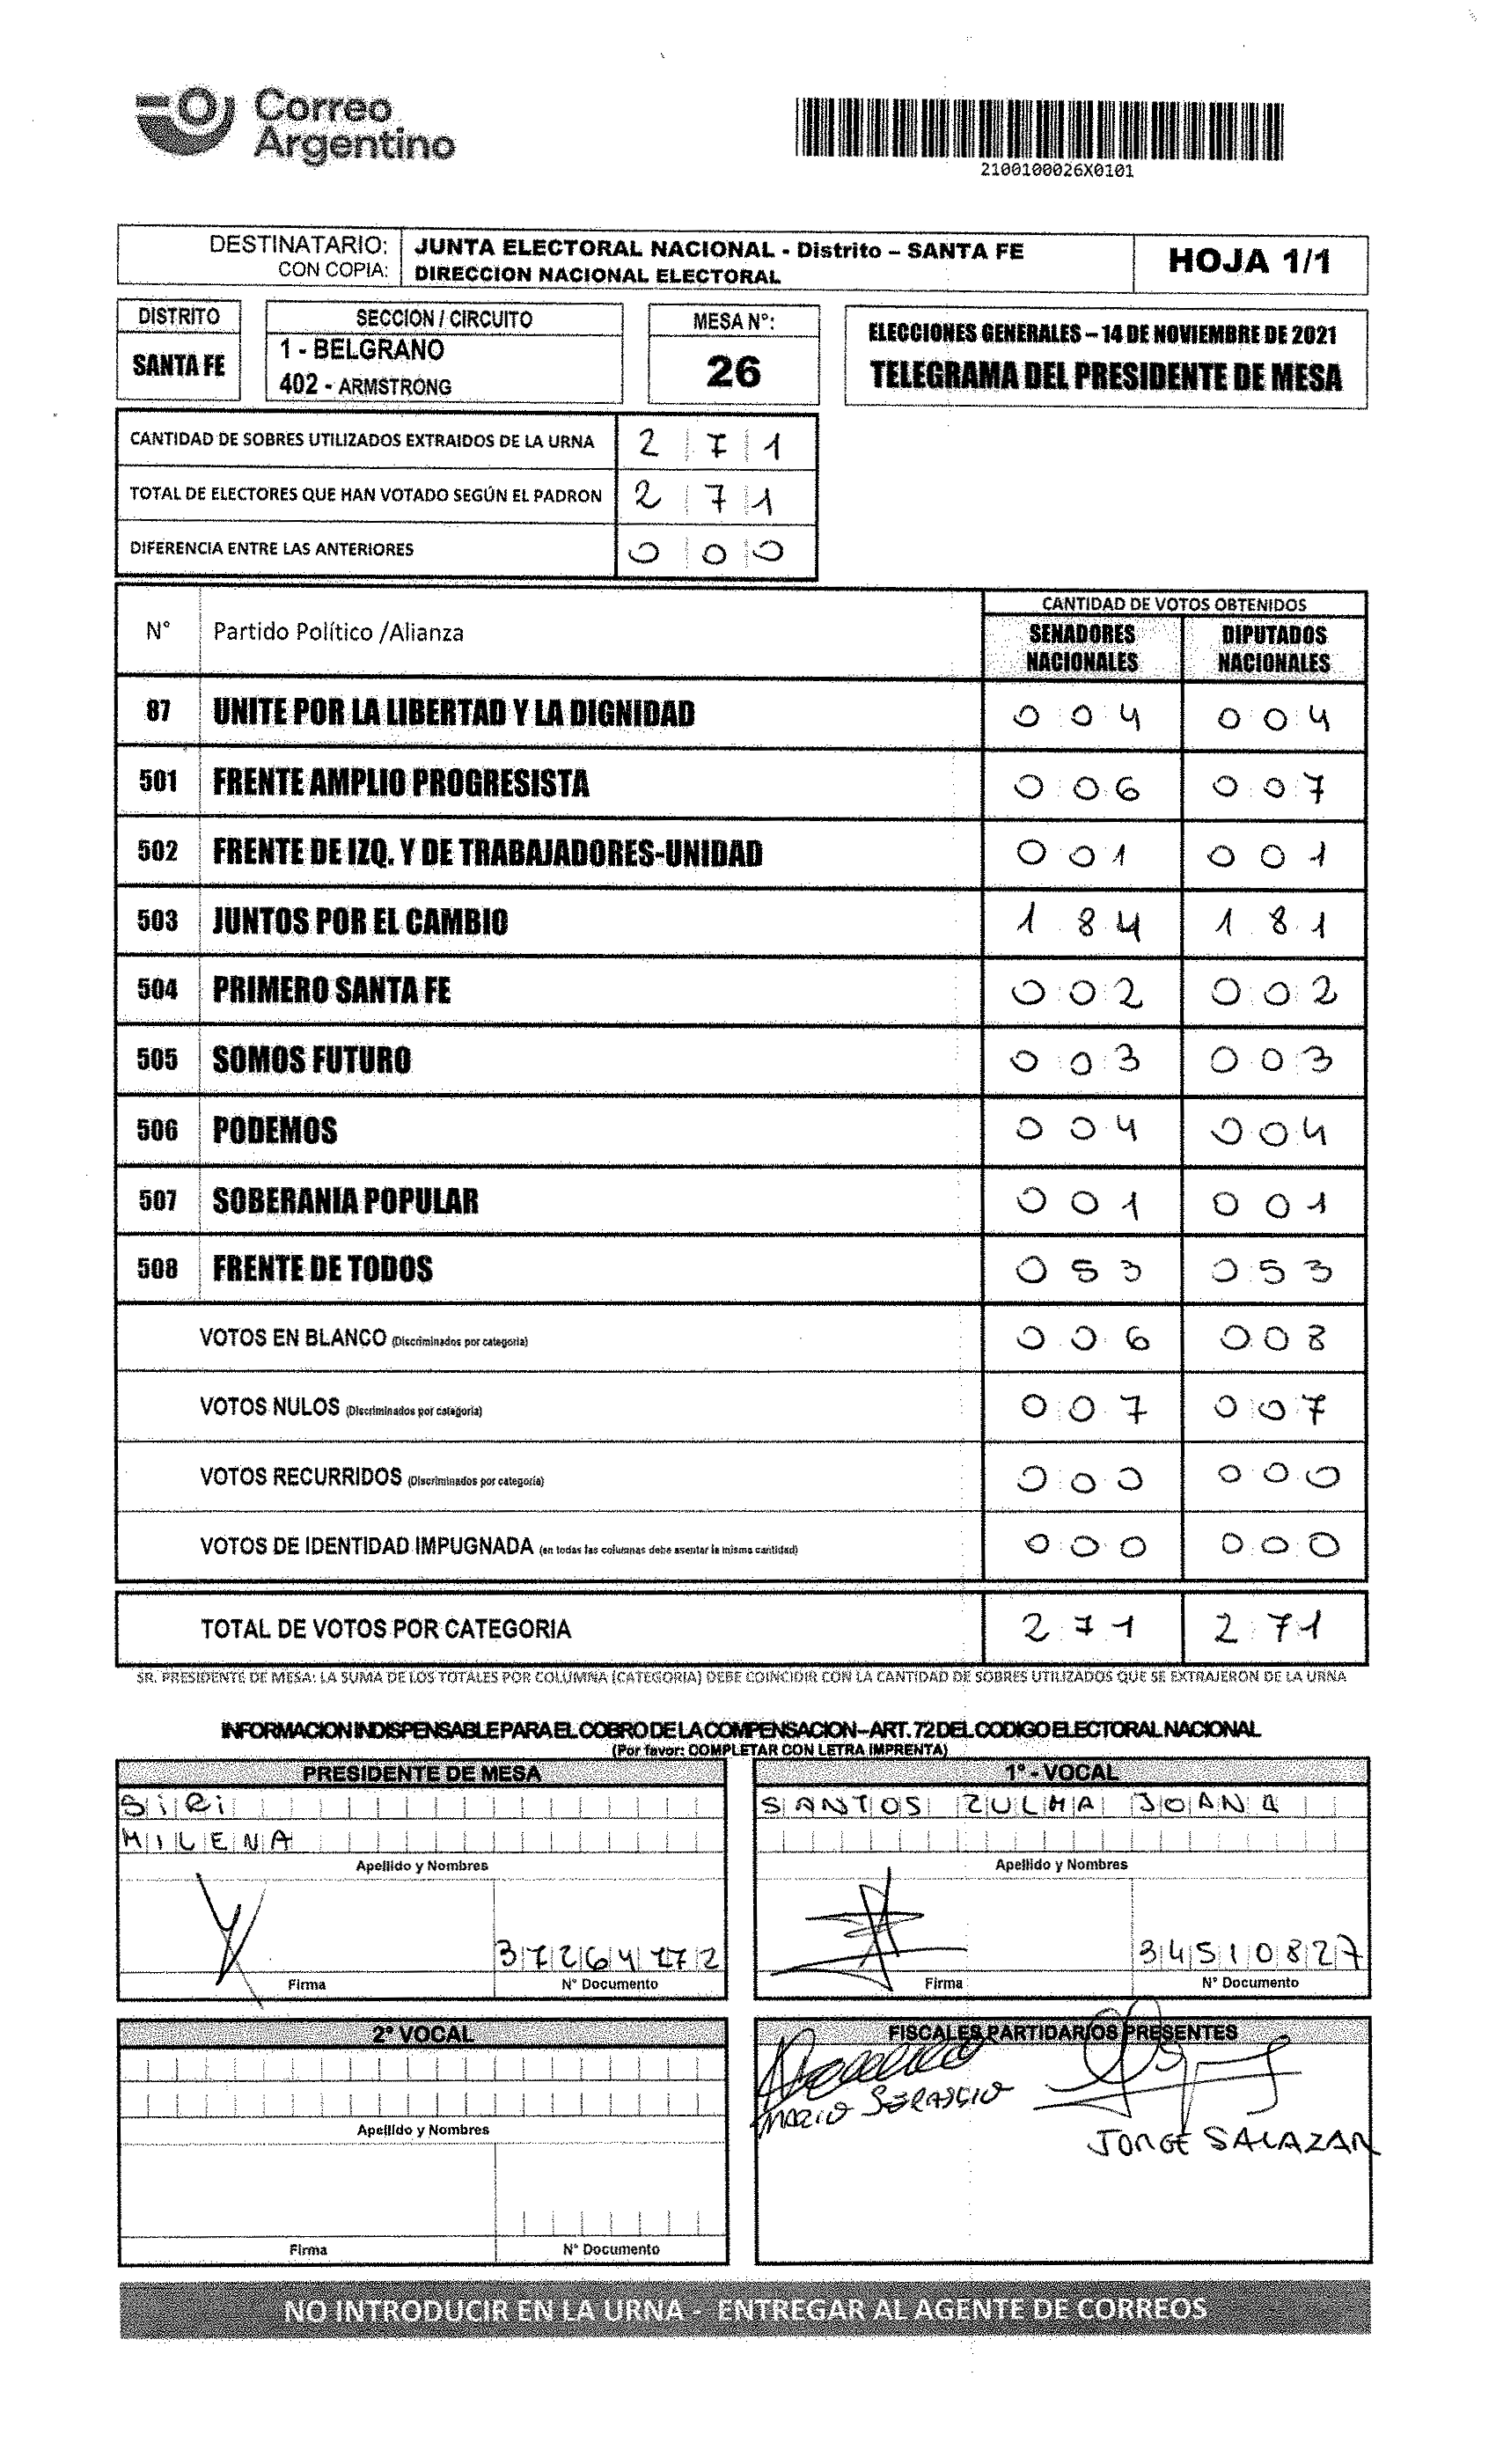
\includegraphics[width=135pt,height=210pt]{chapter3/etl-1-rotacion.png}};
        \draw (90,140) node  {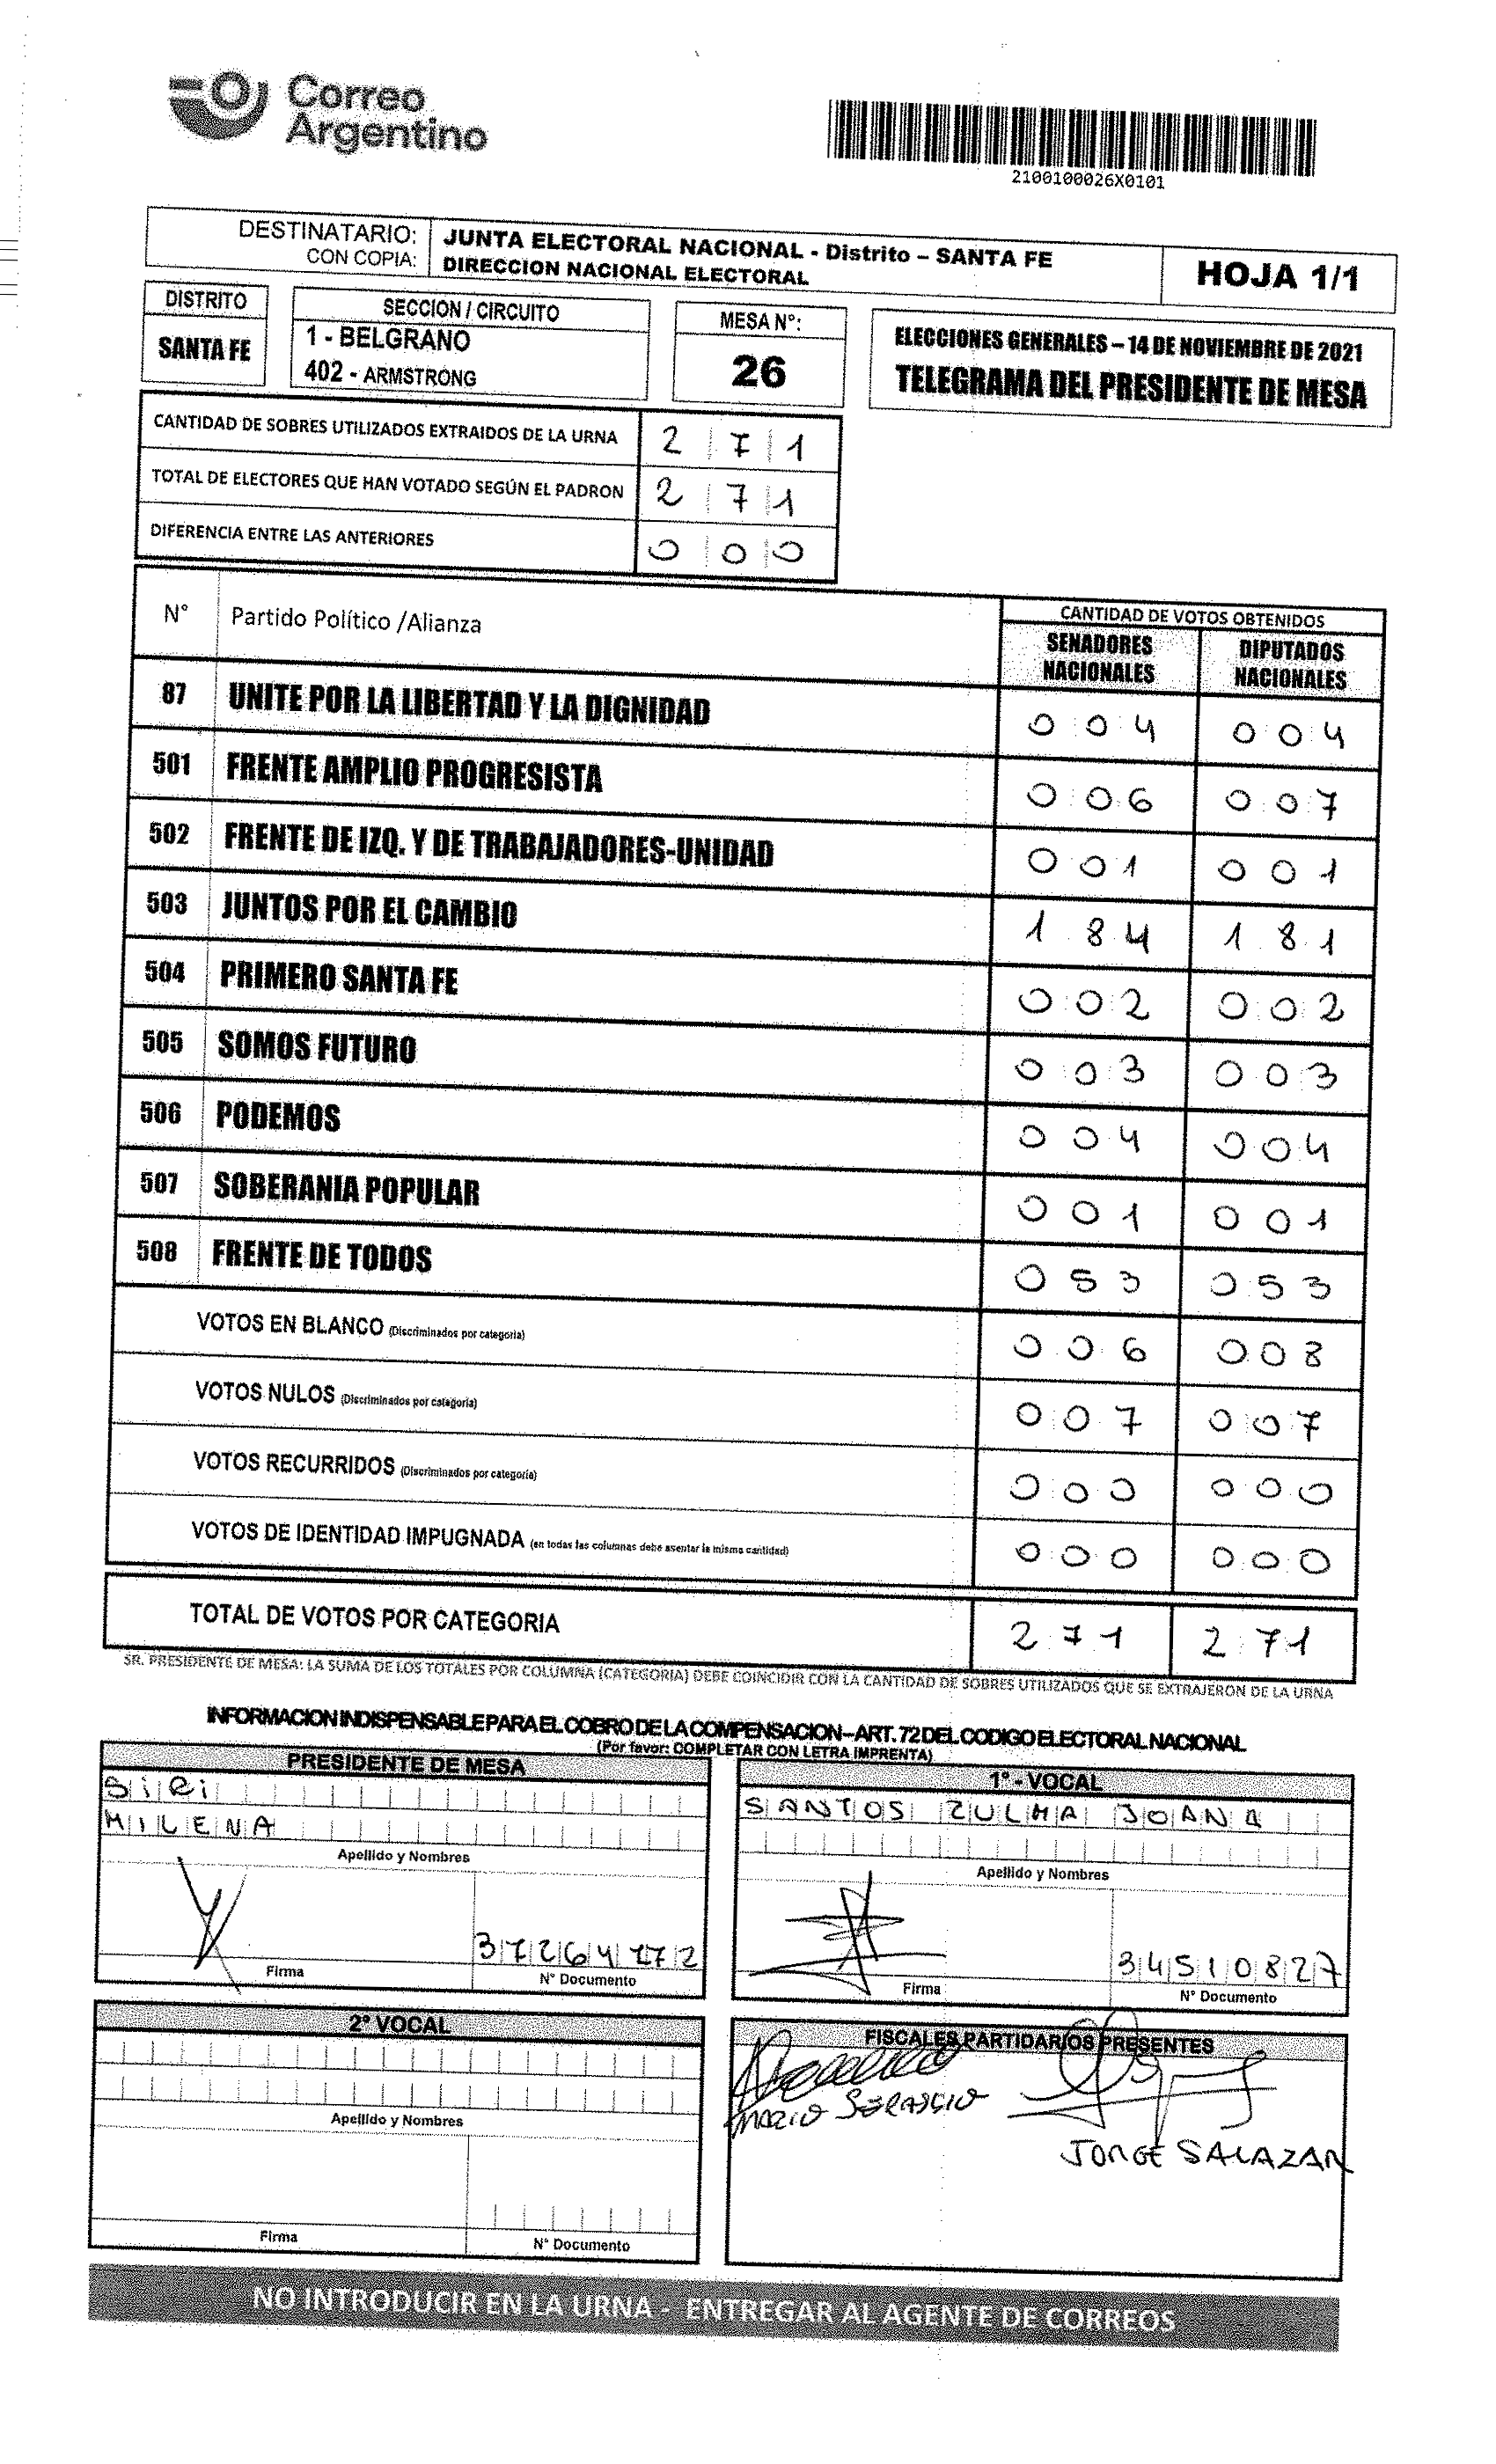
\includegraphics[width=135pt,height=210pt]{chapter3/etl-1-telegrama.png}};
        \draw    (190.8,110.6) -- (267.4,110.6) ;
        \draw [shift={(269.4,110.6)}, rotate = 180] [color={rgb, 255:red, 0; green, 0; blue, 0 }  ][line width=0.75]    (10.93,-3.29) .. controls (6.95,-1.4) and (3.31,-0.3) .. (0,0) .. controls (3.31,0.3) and (6.95,1.4) .. (10.93,3.29)   ;
        \draw (190,87.18) node [anchor=north west][inner sep=0.75pt]   [align=left] {Enderezar};

    \end{tikzpicture}

    \caption{Enderezamiento de un telegrama utilizando OpenCV.}
    \label{fig:etl-1-rotacion}
\end{figure}

\subsection{Extracción de la grilla de votos}
El siguiente paso consiste en poder seleccionar la grilla de los votos y poder extraerla para seguir trabajando en
ella. Esto puede realizarse utilizando la funcion \verb|getContours| de OpenCV y quedándose con el contorno de mayor
área.

\begin{figure}[H]
    \centering
    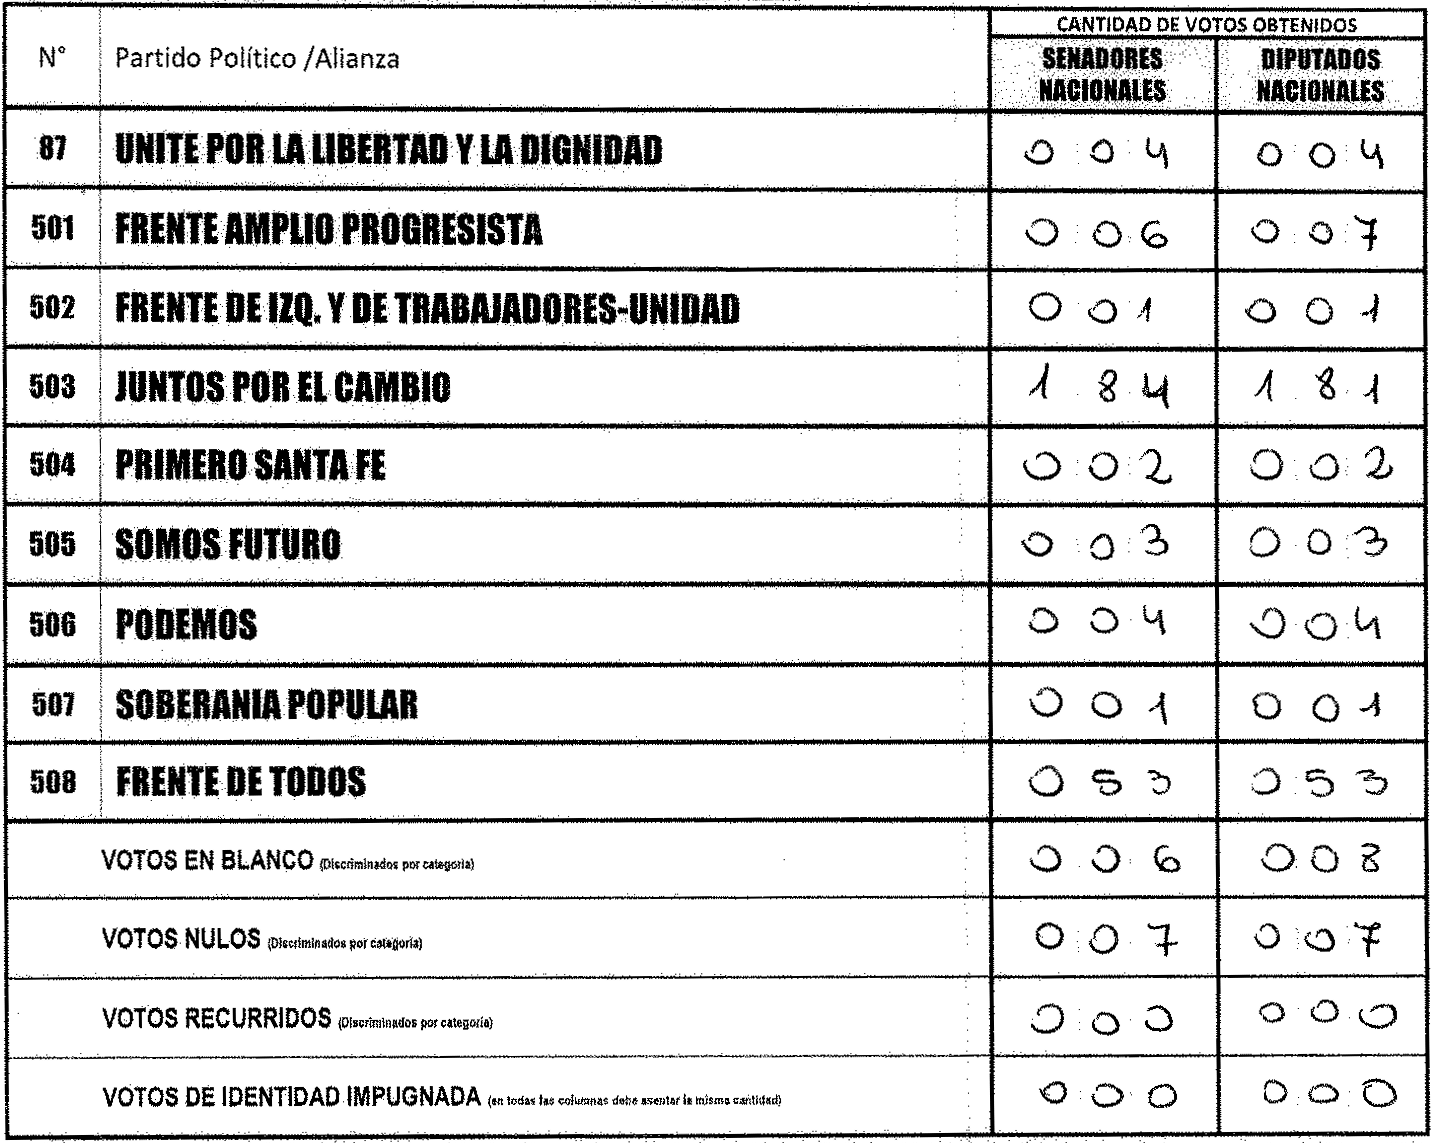
\includegraphics[width=0.4\textwidth, height=0.3\textwidth]{chapter3/etl-2-grilla.png}
    \caption{Grilla de votos extraída buscando el contorno de mayor área.}
    \label{fig:etl-2-grilla}
\end{figure}

\subsection{Detección de líneas de la grilla de votos}
Teniendo la grilla de votos separada del telegrama, se procede a detectar las líneas para poder extraer cada registro
de la misma. Si bien OpenCV posee funciones para la detección de líneas, se optó por utilizar un enfoque simplificado.
El mismo es similar al utilizado en \parencite{lamagna2016lectura}. Debido a que la grilla se encuentra enderezada, se puede utilizar proyecciones de los
colores sobre los ejes $x$ e $y$ para detectarlas. Al sumar todos los colores por eje, se pueden encontrar los picos
donde se encuentran las lineas horizontales y verticales. Posteriormente, se selecciona un umbral de corte por cada
eje, siendo el promedio menos dos desvíos estándar. La figura \ref{fig:etl-3-proyecciones} muestra las proyecciones
obtenidas con los umbrales por cada eje.

\begin{figure}
    \centering

    \tikzset{every picture/.style={line width=0.75pt}}

    \begin{tikzpicture}[x=0.75pt,y=0.75pt,yscale=-1,xscale=1]
        \draw (142.77,162.65) node  {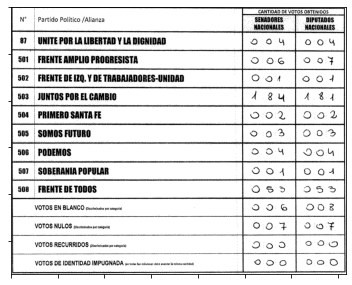
\includegraphics[width=214.16pt,height=173.4pt]{chapter3/etl-3-grilla.png}};
        \draw (303.6,159.11) node [rotate=-90] {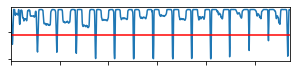
\includegraphics[width=172pt,height=46.15pt]{chapter3/etl-3-grilla-proyeccion-y.png}};
        \draw (142.5,30.77) node  {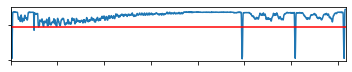
\includegraphics[width=213.75pt,height=46.15pt]{chapter3/etl-3-grilla-proyeccion-x.png}};
    \end{tikzpicture}

    \caption{Proyecciones de los ejes de la grilla. En rojo se marca el umbral de corte.}
    \label{fig:etl-3-proyecciones}
\end{figure}

Sin embargo, aunque se seleccione aquellos pixeles que se encuentren por debajo del umbral, por cada pico existe mas de
un pixel. Siguiendo con el ejemplo, en el eje $x$ se obtienen los siguientes pixeles que se encuentran en los
``picos'':

\begin{verbatim}
    array([    3,    4,    5,    6,    7,  100,  119,  120,  988, 
             989,  990,  991,  992, 1215, 1216, 1217, 1218, 1219, 
            1423, 1424, 1425, 1426, 1427])
\end{verbatim}

Con la estrategia del umbral no se obtienen las 4 líneas que se desean detectar sobre el eje $x$. No obstante, se puede
aplicar un clustering jerárquico sobre los índices obtenidos y luego calcular el índice promedio de cada cluster para
tomarlo como único representante. El proceso se repite de la misma manera sobre el eje $y$. Esta última modificación
sobre el trabajo realizado en \parencite{lamagna2016lectura} asegura tener un único pixel por línea.

\begin{figure}[H]
    \centering
    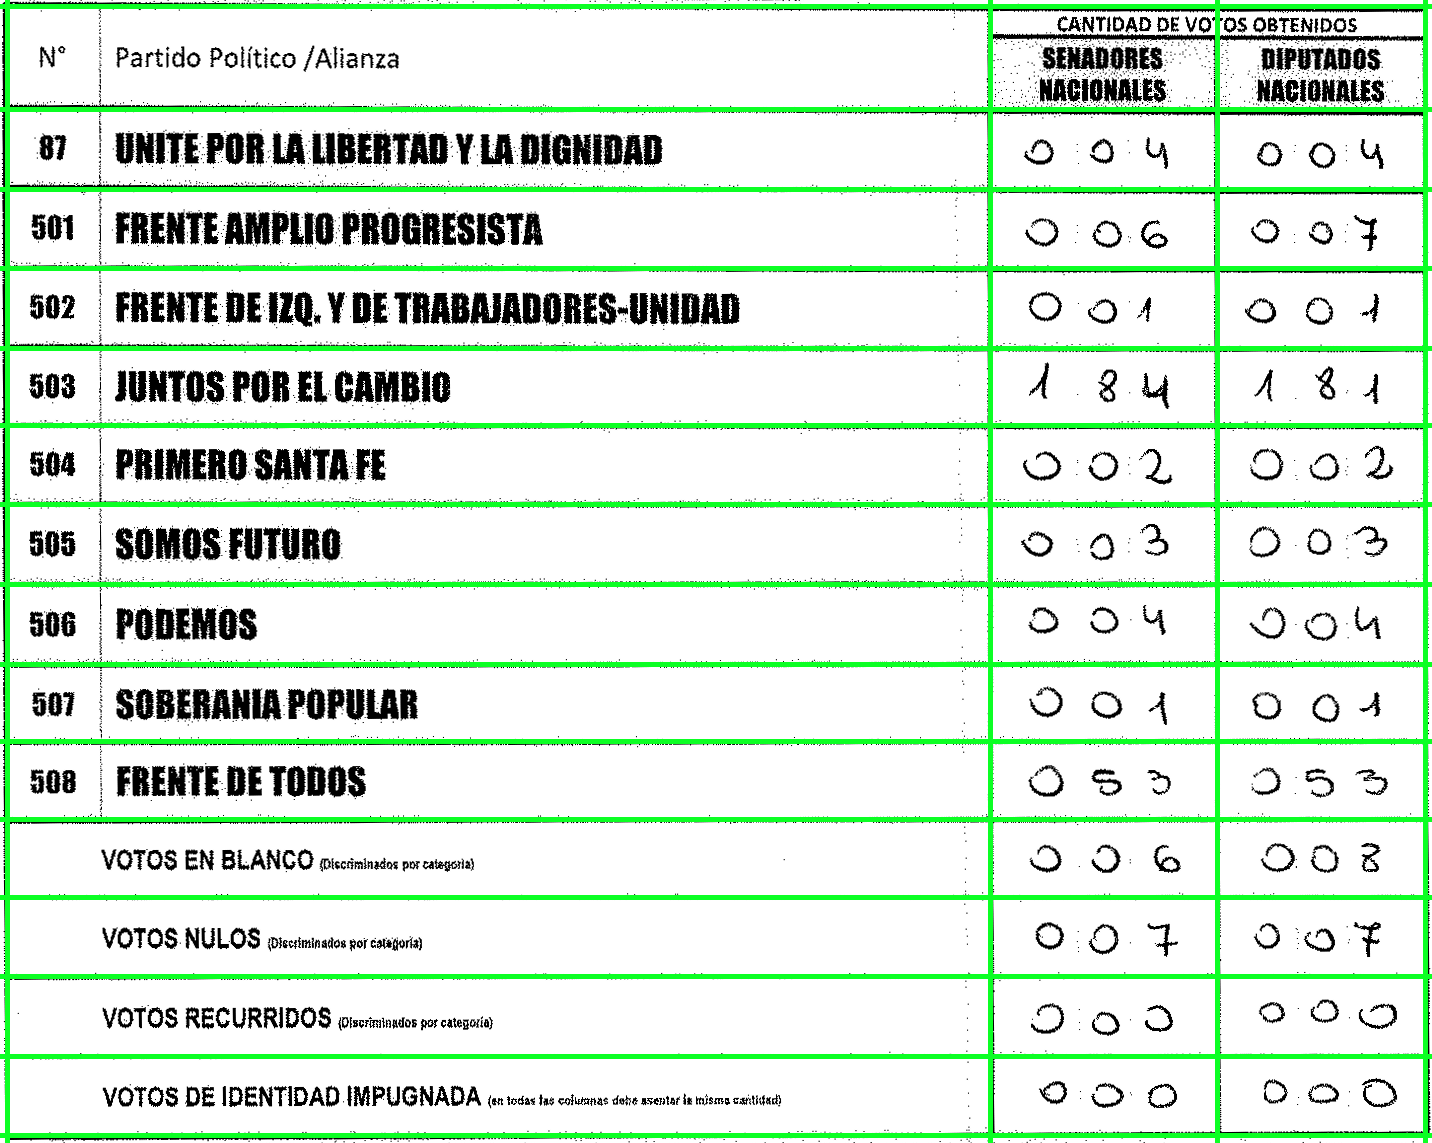
\includegraphics[width=0.4\textwidth, height=0.3\textwidth]{chapter3/etl-3-grilla-detectada.png}
    \caption{Grilla detectada (en verde) utilizando el umbral por sobre las proyecciones y su posterior agrupamiento con clustering jerárquico.}
    \label{fig:etl-3-grilla-detectada}
\end{figure}

\subsection{Segmentación de dígitos}

Una vez obtenida la grilla, se itera por cada registro obteniendo los rectángulos que contienen los votos, ignorando el
primer renglón que contiene los títulos de la grilla.

\begin{figure}[H]
    \centering
    \frame{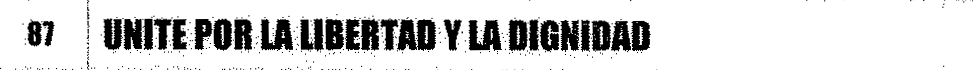
\includegraphics[height=15pt]{chapter3/etl-4-registro-1.png}}
    \frame{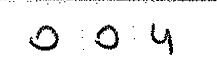
\includegraphics[height=15pt]{chapter3/etl-4-registro-2.png}}
    \frame{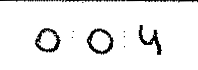
\includegraphics[height=15pt]{chapter3/etl-4-registro-3.png}}
    \caption{Primer registro extraído de la grilla de votos.}
    \label{fig:etl-4-registro}
\end{figure}

Para separar cada dígito en una única imagen, se utiliza un análisis de componentes conectados
(\verb|connectedComponents| de OpenCV) y se recortan aquellos contornos que posean de área entre el $5\%$ y el $70\%$
de los pixeles totales de la imagen. Los valores fueron obtenidos mediante experimentación y sirven para descartar
ruido que pueda detectar el análisis de componentes conectados.

\begin{figure}[H]
    \centering
    \frame{
\includegraphics[scale=0.6]{chapter3/etl-4-digito-1.png}}
    \frame{
\includegraphics[scale=0.6]{chapter3/etl-4-digito-2.png}}
    \frame{
\includegraphics[scale=0.6]{chapter3/etl-4-digito-3.png}}
    \caption{Dígitos detectados en el primer bloque de votos.}
    \label{fig:etl-4-digitos}
\end{figure}

Por último, los dígitos son encuadrados y se guardan junto al partido político y al tipo de voto (senadores o
diputados) en un dataset, cuyo análisis será abordado en la siguiente sección.

\section{Análisis del dataset}

Con la extracción descripta en la sección anterior, se procede a hacer un análisis exploratorio de los datos en
búsqueda de posibles errores. La tabla \ref{tab:dataset-telegramas-segmentados} muestra algunos registros del dataset
que vincula los dígitos extraídos de los telegramas con los partidos políticos.

\begin{table}[H]
    \centering
    \begin{tabular}{ccccc}
        \toprule
        Telegrama                                                               & Partido         & Tipo      & Dígitos                                                                  & \# Dígitos \\
        \midrule
        2100100026X                                                             & Unite           & Diputados & \frame{
\includegraphics[scale=0.6]{chapter3/eda/unite-diputados-1.png}}
        \frame{
\includegraphics[scale=0.6]{chapter3/eda/unite-diputados-2.png}}
        \frame{
\includegraphics[scale=0.6]{chapter3/eda/unite-diputados-3.png}} & 3                                                                                                                   \\
        2100100026X                                                             & Unite           & Senadores & \frame{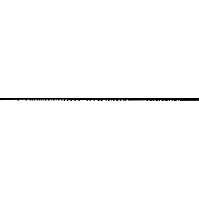
\includegraphics[scale=0.08]{chapter3/eda/unite-senadores-1.png}}
        \frame{
\includegraphics[scale=0.6]{chapter3/eda/unite-senadores-2.png}}
        \frame{
\includegraphics[scale=0.6]{chapter3/eda/unite-senadores-3.png}}
        \frame{
\includegraphics[scale=0.6]{chapter3/eda/unite-senadores-4.png}} & 4                                                                                                                   \\
        2100100067X                                                             & Frente de Todos & Diputados & \frame{
\includegraphics[scale=0.6]{chapter3/eda/todos-diputados-1.png}}
        \frame{
\includegraphics[scale=0.6]{chapter3/eda/todos-diputados-2.png}}
        \frame{
\includegraphics[scale=0.6]{chapter3/eda/todos-diputados-3.png}}
        \frame{
\includegraphics[scale=0.6]{chapter3/eda/todos-diputados-4.png}} & 4                                                                                                                   \\
        2100100067X                                                             & Frente de Todos & Senadores & \frame{
\includegraphics[scale=0.6]{chapter3/eda/todos-senadores-1.png}}
        \frame{
\includegraphics[scale=0.6]{chapter3/eda/todos-senadores-2.png}}
        \frame{
\includegraphics[scale=0.6]{chapter3/eda/todos-senadores-3.png}} & 3                                                                                                                   \\
        \bottomrule

    \end{tabular}
    \caption{Ejemplo de registros del dataset. Cada fila representa un voto.}
    \label{tab:dataset-telegramas-segmentados}
\end{table}

El lector podrá darse cuenta que existen errores en el cuadro anterior. En primer lugar, en la columna donde sólamente
deben haber las imágenes de los dígitos existe una con una línea en el segundo registro. Por otro lado, también existen
dígitos mal escritos como los que se encuentran en los dos últimos registros. Para limpiar estas extracciones
incorrectas, se calculan dos columnas las cuales contienen las proporciones mínimas y máximas de pixeles blancos en las
imágenes por cada voto. La figura \ref{fig:histogramas-min-max-prop-blanco} muestra los histogramas generales de las
mismas.

\begin{figure}[H]
    \centering
    \begin{subfigure}[h]{0.48\textwidth}
        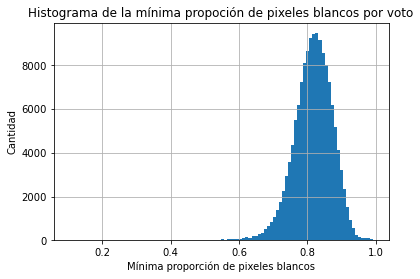
\includegraphics[width=1\textwidth]{chapter3/eda/hist-min-prop-blanco.png}
        \caption{Histograma de la proporción mínima de pixeles blancos en un voto.}
        \label{fig:histograma-min-prop-blanco}
    \end{subfigure}
    \hfill
    \begin{subfigure}[h]{0.48\textwidth}
        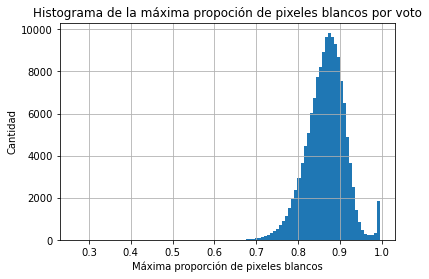
\includegraphics[width=1\textwidth]{chapter3/eda/hist-max-prop-blanco.png}
        \caption{Histograma de la proporción máxima de pixeles blancos en un voto.}
        \label{fig:histograma-max-prop-blanco}
    \end{subfigure}
    \caption{Histogramas de proporciones de pixeles blancos por voto.}
    \label{fig:histogramas-min-max-prop-blanco}
\end{figure}

La cola derecha de la distribución de \ref{fig:histograma-max-prop-blanco} presenta un pico anormal en el extremo
cercano a 1. Al eliminar aquellas imágenes de dígitos que posean mas de un $95\%$ de pixeles blancos, se logran
descartar los casos de líneas como la vista en el cuadro \ref{tab:dataset-telegramas-segmentados}. Por el contrario, al
eliminar aquellas imágenes que posean menos del $50\%$ de pixeles blancos, se logran descartar los casos de escritura
incorrecta.

El siguiente punto a analizar es el tamaño de las imágenes. Como fue mostrado en el cuadro
\ref{tab:dataset-telegramas-segmentados}, las imágenes no fueron estandarizadas en un tamaño estándar. De manera
análoga a la variable de proporción de pixeles blancos, se calculan las variables mínimo y máximo tamaño por voto. La
tabla \ref{tab:describe-min-max-size} muestra los estadísticos descriptivos de las mismas.

\begin{table}[H]
    \centering
    \begin{tabular}{crrrrr}
        \toprule
        Variable      & Promedio & Desvío & Mínimo & Mediana & Máximo \\
        \midrule
        Tamaño mínimo & 38.35    & 9.61   & 13     & 37      & 621    \\
        Tamaño máximo & 44.80    & 10.73  & 18     & 43      & 621    \\
        \bottomrule
    \end{tabular}
    \caption{Estadísticos descriptivos del mínimo y máximo tamaño de las imágenes de los votos.}
    \label{tab:describe-min-max-size}
\end{table}

Al analizar los valores extremos, se encuentran telegramas que fueron cargados de forma incorrecta (ver anexo
\ref{anexo:telegrama-erroneo}) o con caligrafía en la cual los números se encuentran unidos y no pueden ser separados
por el análisis de componentes conectados de OpenCV (ver anexo \ref{anexo:telegrama-numeros-juntos}). Se eliminan estos
casos filtrando por aquellos registros que se encuentren por fuera de la media +- 4 desvíos estándar.

Concluida la etapa de análisis y limpieza, se exportan los dígitos en un formato similar al dataset {\it MNIST} con la
etiqueta que oficialmente fue registrada en las elecciones del 2021. El mismo será nombrado como {\it TDS} (dataset de
telegramas) de aquí en adelante. El mismo posee un total de 170.718 imágenes de dígitos cuadradas con sus dimensiones
orginales, es decir, no se encuentran estandarizados en una dimension específica. Esto último es adrede ya que puede
servir para mejorar el dataset en futuros trabajos.

\begin{figure}[H]
    \centering
    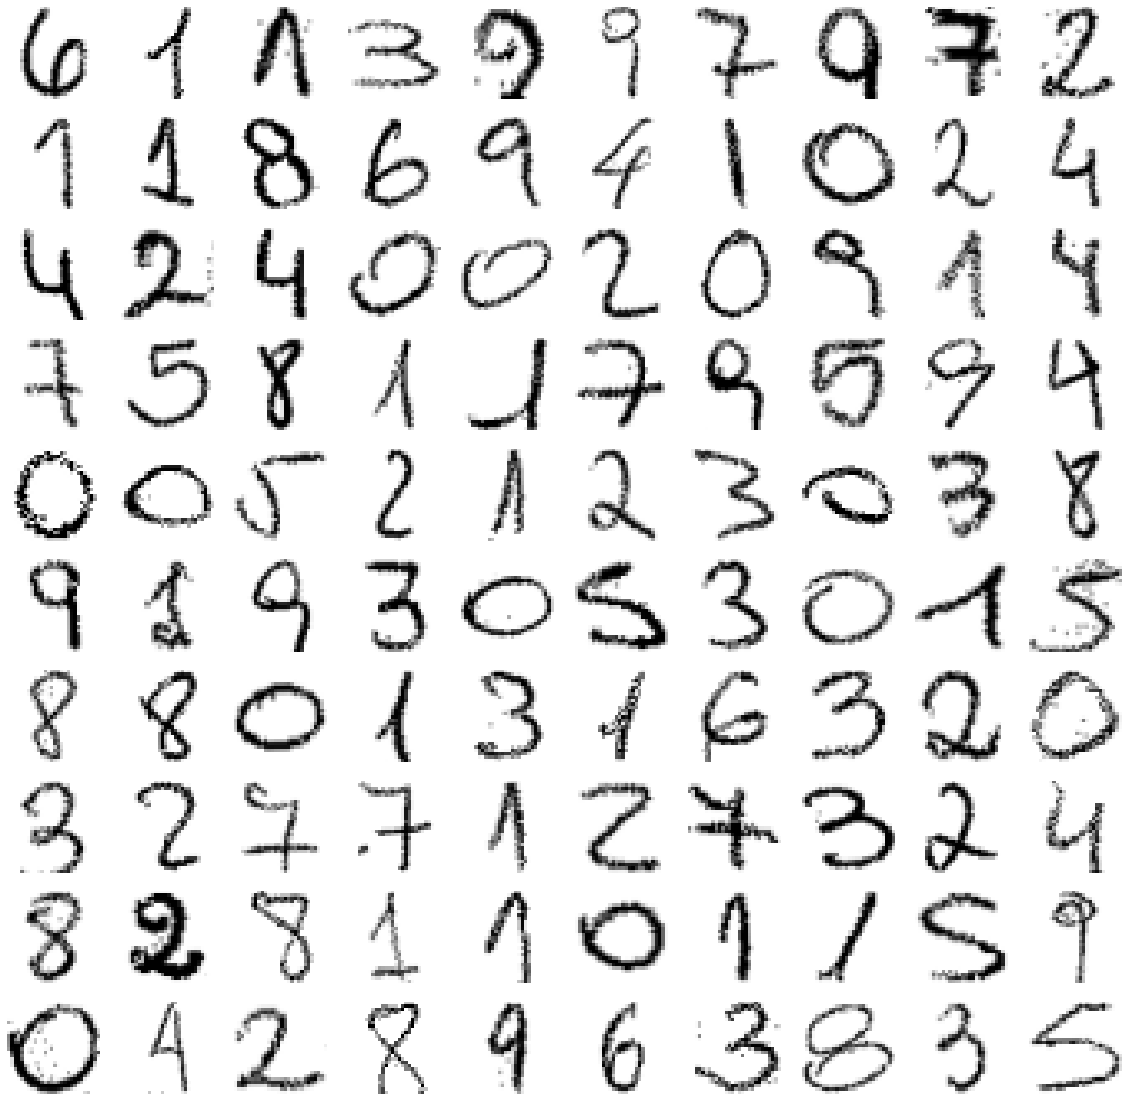
\includegraphics[width=0.5\textwidth]{chapter3/tds.png}
    \caption{Dataset TDS de dígitos.}
    \label{fig:tds}
\end{figure}

\section{Diseño experimental}

Los experimentos fueron programados en Python mediante la librería PyTorch \parencite{NEURIPS2019_9015} y TLLIB \parencite{tllib} para aplicar las técnicas de adaptación de dominio.

Se entrenaron redes ResNet-50 \parencite{he2016deep} y LeNet-8 \parencite{lecun1998gradient} por cada una de las técnicas de adaptación de dominio descriptas en el capítulo
\ref{Chapter2}. Como modelo baseline, se entrenaron ambas redes sin ninguna técnica de adaptación.

\subsection{Metodología de entrenamiento}

Para entrenar modelos mediante adaptación de dominio, se precisan dos datasets: el de origen que se encuentra
etiquetado y el de destino sin etiquetar. Los experimentos llevados a cabo utilizan el {\it MNIST} como origen y el
    {\it TDS} como destino. En cada iteración de entrenamiento, se provee de un batch de 1024 imágenes del dataset origen y
otro del de destino. Se realizaron 3 particiones de cada uno:

\begin{itemize}
    \item Entrenamiento (70\% de cada dataset): utilizado para entrenar la LeNet-8 y ResNet-18 en cada época.
    \item Validación (15\% de cada dataset): utilizado para calcular los mejores hiperparámetros del modelo.
    \item Test (15\% de cada dataset): utilizado para calcular las métricas y gráficos finales del modelo entrenado.
\end{itemize}

Los modelos se entrenaron utilizando Stochastic Gradient Descent (SGD) \parencite{sutskever2013importance} utilizando nesterov, 0.9 como momento y 0.001 de weight decay.

\subsection{Selección y optimización del modelo}

La optimización de hiperparámetros se realizó utilizando la librería Optuna \parencite{optuna_2019}. Se ejecutaron 30 rondas de optimización con 10 épocas de entrenamiento por cada experimento. En
cada uno de los experimentos, se optimizaron los hiperparámetros para minimizar el loss de cada modelo. El cuadro
\ref{tab:rangos-hiperparametros} muestra los rangos búsqueda.

\begin{table}[H]
    \centering
    \begin{tabular}{l|cccccc}
        \toprule
                   & {\it DANN}  & {\it ADDA}  & {\it DANN+BSP} & {\it MDD}   & {\it AFN}    & {\it Sin AD} \\
        \midrule
        $\eta_0$   & [1e-4, 0.1] & [1e-4, 0.1] & [1e-4, 0.1]    & [1e-4, 0.1] & [1e-4, 0.1]  & [1e-4, 0.1]  \\
        $\lambda$  & [0.5, 2]    & [0.5, 2]    & [0.5, 2]       & [0.5, 2]    & [0.001, 0.1] & -            \\
        $\beta$    & -           & -           & [1e-5, 0.1]    & -           & [0.0, 0.1]   & -            \\
        $\gamma$   & -           & -           & -              & [1, 10]     & -            & -            \\
        $\Delta_r$ & -           & -           & -              & -           & [0.01, 5]    & -            \\
        \# Blocks  & -           & -           & -              & -           & [1, 4]       & -            \\
        Dropout    & -           & -           & -              & -           & [0.3, 0.7]   & -            \\
        \bottomrule
    \end{tabular}
    \caption{Rango de hiperparámetros optimizados. $^{*}$LR refiere a ``learning rate''. $^{**}$T-O refiere a ``trade-off''.}
    \label{tab:rangos-hiperparametros}
\end{table}

Se implementó una disminución del learning rate en cada iteración de cada época, mediante la fórmula
\ref{eq:learning-rate}. Se mantuvieron constantes los valores de $\gamma=0.001$ y $\theta = 0.25$.

\begin{equation}
    \eta(t) = \eta_0 * (1 + \gamma * t)^{-\theta}
    \label{eq:learning-rate}
\end{equation}

\section{Métricas de evaluación}

Los modelos optimizados serán evaluados con distintas métricas en tiempo de test, descriptas en las siguientes
sub-secciones del capítulo. Las mismas pretenden evaluar qué tan buenos son los modelos respecto a la tarea de
clasificación y qué capacidad de adaptación de dominio poseen.

\subsection{Métricas de clasificación}
\subsubsection{Accuracy}

La métrica de {\it accuracy} permite identificar qué tan cerca o lejos un conjunto de observaciones se encuentra
respecto a los valores reales. Es el ratio de predicciones correctas sobre las totales.

\begin{equation}
    Accuracy(y, \hat{y}) = \frac{1}{n} \sum_{i=0}^{n-1} 1(\hat{y_{i}}=y_{i})
\end{equation}

Donde:
\begin{itemize}
    \item $n$: es la cantidad de observaciones totales.
    \item $y_{i}$: es el valor de la ${i}$-ésima observación correspondiente al real.
    \item $\hat{y_{i}}$: es el valor predicho para la ${i}$-ésima observación.
    \item $1(x)$: es la función indicador.
\end{itemize}

\subsubsection{$F_{1}$}

La métrica $F_{1}$ es una media armónica de otras dos: {\it precisión} y {\it recall}. De manera simplificada, la
primera muestra la capacidad del modelo de no etiquetar como positivo una obsevación que es negativa y la segunda
muestra la capacidad del modelo de encontrar todas las observaciones positivas.

La {\it precisión} consiste en calcular el ratio de predicciones positivas correctas de la clase respecto al total de
predicciones positivas de la clase.

\begin{equation}
    Precision(y, \hat{y}) = \frac{TP}{TP + FP}
\end{equation}

Donde:
\begin{itemize}
    \item $TP$: es la cantidad de verdaderos positivos.
    \item $FP$: es la cantidad de falsos positivos.
\end{itemize}

Por otro lado, el {\it recall} consiste en calcular el ratio de predicciones positivas correctas de la clase respecto
al total de predicciones correctas de la clase.

\begin{equation}
    Recall(y, \hat{y}) = \frac{TP}{TP + FN}
\end{equation}

Donde:
\begin{itemize}
    \item $TP$: es la cantidad de verdaderos positivos.
    \item $FN$: es la cantidad de falsos negativos.
\end{itemize}

Las dos métricas mencionada anteriormente pueden ser combinadas en una sola denominada $F_{\beta}$. El valor de $\beta$
permite asignar un peso distinto a la precisión o al recall dentro del promedio armónico. Cuando $\beta=1$, ambas
poseen el mismo peso.

\begin{equation}
    F_{\beta}(y, \hat{y}) = (1 + \beta^2) \times \frac{precision(y, \hat{y}) \times recall(y, \hat{y})}{\beta^2 \times precision(y, \hat{y}) + recall(y, \hat{y})}
\end{equation}

El rango de valores es de $[0, 1]$, donde 1 corresponde a un clasificador que funciona sin errores.

\subsubsection{Intersección sobre unión}

Otra forma de medir el clasificador es mediante la {\it intersección sobre unión} (IoU por sus siglas en inglés).
Consta de calcular la cantidad de dígitos únicos predichos por sobre la cantidad de dígitos únicos reales. Por ejemplo,
para un telegrama y un partido el clasificador predice 189 votos cuando lo real es 180. Entonces, el {\it IoU} viene
dado por:

\begin{align}
    IoU(\{1, 8, 0\}, \{1, 8, 9\}) & = \frac{\lvert\{1, 8, 0\} \bigcap \{1, 8, 9\}\rvert}{\lvert\{1, 8, 0\} \bigcup \{1, 8, 9\}\rvert} \nonumber \\
                                  & = \frac{\lvert\{1, 8\}\rvert}{\lvert\{1, 8, 0, 9\}\rvert}                                         \nonumber \\
                                  & = \frac{2}{4}                                                                     \nonumber                 \\
                                  & = 0.5
\end{align}

De forma general: sea $y_{i}$ el dígito $i$-ésimo del voto real $y$ de longitud $n$, $\hat{y_{j}}$ el dígito $j$-ésimo
del voto predicho por el modelo $\hat{y}$ de longitud $m$, entonces la métrica viene dada por:

\begin{equation}
    IoU(y, \hat{y}) = \frac{\lvert \{y_{i}\} \bigcap \{\hat{y_{j}}\}\rvert}{\lvert \{y_{i}\} \bigcup \{\hat{y_{j}}\}\rvert} \forall i \in \{1, \cdots, n\}, \forall j \in \{1, \cdots, m\}
\end{equation}

\subsection{Métricas de adaptación}
\subsubsection{Distancia $\mathcal{A}$}

La distancia $\mathcal{A}$ mide la similaridad entre dos distribuciones. Puede ser utilizada para analizar los espacios
latentes de clasificadores en problemas de adaptación de dominio \parencite{ben2006analysis}. La métrica viene dada por:

\begin{equation}
    dist_\mathcal{A} = 2 (1-2\epsilon)
\end{equation}

Donde $\epsilon$ es el error en test de un clasificador entrenado para discriminar el dominio de origen del de destino.
Cuando el error de clasificación es bajo, significa que hay diferencias significativas entre las dos distrubiones,
haciendo que $dist_\mathcal{A}$ sea grande y vice versa.

En la figura \ref{fig:ejemplos-dist-a} se muestran posibles casos de distribuciones de dominios. En la sub-figura
\ref{fig:dominios-distintos} las distribuciones de dominios son significativamente diferentes entre si, por lo tanto
$dist_\mathcal{A} \approx 2$. Por el contrario, en la sub-figura \ref{fig:dominios-similares} las distribuciones de
dominios son similares entre si, por lo que se espera que $dist_\mathcal{A} \approx 0$.

\begin{figure}[H]
    \centering
    \begin{subfigure}[h]{0.46\textwidth}
        \centering
        \tikzset{every picture/.style={line width=0.75pt}}
        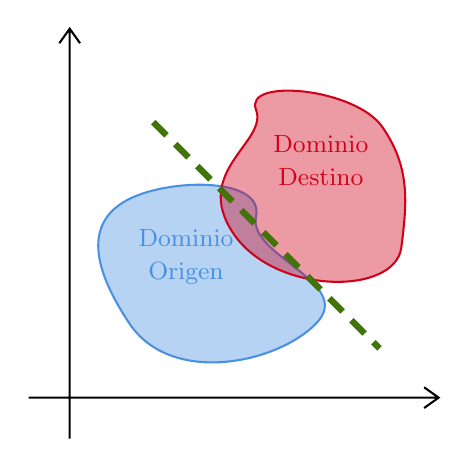
\begin{tikzpicture}[x=0.75pt,y=0.75pt,yscale=-1,xscale=1]
            \draw  (0,177.75) -- (197.5,177.75)(19.75,0) -- (19.75,197.5) (190.5,172.75) -- (197.5,177.75) -- (190.5,182.75) (14.75,7) -- (19.75,0) -- (24.75,7)  ;
            \draw  [color={rgb, 255:red, 74; green, 144; blue, 226 }  ,draw opacity=1 ][fill={rgb, 255:red, 74; green, 144; blue, 226 }  ,fill opacity=0.4 ] (48.5,82) .. controls (68.5,72) and (113.5,71.5) .. (109.5,90.5) .. controls (105.5,109.5) and (157.5,122.5) .. (138.5,142) .. controls (119.5,161.5) and (68.5,172) .. (48.5,142) .. controls (28.5,112) and (28.5,92) .. (48.5,82) -- cycle ;
            \draw  [color={rgb, 255:red, 208; green, 2; blue, 27 }  ,draw opacity=1 ][fill={rgb, 255:red, 208; green, 2; blue, 27 }  ,fill opacity=0.4 ] (109.5,39) .. controls (103.5,23.5) and (157.5,28.5) .. (170.5,47.5) .. controls (183.5,66.5) and (182.5,82.5) .. (179.5,105.5) .. controls (176.5,128.5) and (118.5,128.5) .. (98.5,98.5) .. controls (78.5,68.5) and (115.5,54.5) .. (109.5,39) -- cycle ;
            \draw (115,50) node [anchor=north west][inner sep=0.75pt]  [color={rgb, 255:red, 208; green, 2; blue, 27 }  ,opacity=1 ] [align=left] {\begin{minipage}[lt]{36.4pt}\setlength\topsep{0pt}
                    \begin{center}
                        {\small Dominio}\\{\small Destino}
                    \end{center}

                \end{minipage}};
            \draw (50,95) node [anchor=north west][inner sep=0.75pt]  [color={rgb, 255:red, 74; green, 144; blue, 226 }  ,opacity=1 ] [align=left] {\begin{minipage}[lt]{36.4pt}\setlength\topsep{0pt}
                    \begin{center}
                        {\small Dominio}\\{\small Origen}
                    \end{center}

                \end{minipage}};
            \draw [color={rgb, 255:red, 65; green, 117; blue, 5 }  ,draw opacity=1 ][line width=2.25]  [dash pattern={on 6.75pt off 4.5pt}]  (60,45) -- (169,154) ;
        \end{tikzpicture}
        \caption{Dominios distintos, discriminables.}
        \label{fig:dominios-distintos}
    \end{subfigure}
    \hfill
    \begin{subfigure}[h]{0.46\textwidth}
        \centering
        \tikzset{every picture/.style={line width=0.75pt}}

        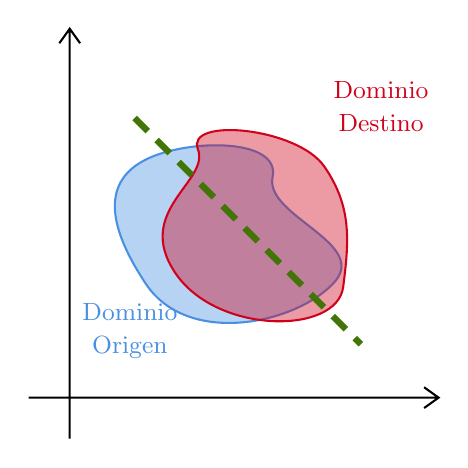
\begin{tikzpicture}[x=0.75pt,y=0.75pt,yscale=-1,xscale=1]
            \draw  (1,179.75) -- (198.5,179.75)(20.75,2) -- (20.75,199.5) (191.5,174.75) -- (198.5,179.75) -- (191.5,184.75) (15.75,9) -- (20.75,2) -- (25.75,9)  ;
            \draw  [color={rgb, 255:red, 74; green, 144; blue, 226 }  ,draw opacity=1 ][fill={rgb, 255:red, 74; green, 144; blue, 226 }  ,fill opacity=0.4 ] (57.5,65) .. controls (77.5,55) and (122.5,54.5) .. (118.5,73.5) .. controls (114.5,92.5) and (166.5,105.5) .. (147.5,125) .. controls (128.5,144.5) and (77.5,155) .. (57.5,125) .. controls (37.5,95) and (37.5,75) .. (57.5,65) -- cycle ;
            \draw  [color={rgb, 255:red, 208; green, 2; blue, 27 }  ,draw opacity=1 ][fill={rgb, 255:red, 208; green, 2; blue, 27 }  ,fill opacity=0.4 ] (82.5,60) .. controls (76.5,44.5) and (130.5,49.5) .. (143.5,68.5) .. controls (156.5,87.5) and (155.5,103.5) .. (152.5,126.5) .. controls (149.5,149.5) and (91.5,149.5) .. (71.5,119.5) .. controls (51.5,89.5) and (88.5,75.5) .. (82.5,60) -- cycle ;
            \draw [color={rgb, 255:red, 65; green, 117; blue, 5 }  ,draw opacity=1 ][line width=2.25]  [dash pattern={on 6.75pt off 4.5pt}]  (52,45) -- (161,154) ;

            \draw (24,133) node [anchor=north west][inner sep=0.75pt]  [color={rgb, 255:red, 74; green, 144; blue, 226 }  ,opacity=1 ] [align=left] {\begin{minipage}[lt]{36.4pt}\setlength\topsep{0pt}
                    \begin{center}
                        {\small Dominio}\\{\small Origen}
                    \end{center}

                \end{minipage}};
            \draw (145,26) node [anchor=north west][inner sep=0.75pt]  [color={rgb, 255:red, 208; green, 2; blue, 27 }  ,opacity=1 ] [align=left] {\begin{minipage}[lt]{36.4pt}\setlength\topsep{0pt}
                    \begin{center}
                        {\small Dominio}\\{\small Destino}
                    \end{center}

                \end{minipage}};
        \end{tikzpicture}

        \caption{Dominios similares, no discriminables.}
        \label{fig:dominios-similares}
    \end{subfigure}

    \caption{Ejemplos de distribuciones de dominios.}
    \label{fig:ejemplos-dist-a}
\end{figure}

Durante el proyecto se utiliza como clasificador una regresión logística a fin de calcular la distancia $\mathcal{A}$.

\subsubsection{Discrepancia de Medias Máxima}

La discrepancia de medias máxima (MMD por sus siglas en inglés) es una prueba estadística basada en {\it kernels} que
se utiliza para determinar si dos distribuciones dadas son iguales midiendo la distancia entre ellas \parencite{gretton2012kernel}. Dadas las distribuciones $P$ y $Q$ sobre un conjunto $\mathcal{X}$ y un mapa de
características $\phi : \mathcal{X} \rightarrow \mathcal{H}$ donde $\mathcal{H}$ es un conjunto de destino, MMD se
define como:

\begin{align}
    MMD^2(P, Q) = \left\lVert \mathbb{E}_{\mathbf{x} \sim P}[\phi(\mathbf{x})] - \mathbb{E}_{\mathbf{y} \sim Q}[\phi(\mathbf{y})]\right\rVert_{\mathcal{H}}^2
    \label{eq:mmd}
\end{align}

Por ejemplo, si el mapa de características es $\phi(x)=x$ y $\mathcal{X}=\mathcal{H}=\mathbb{R}^d$, MMD se calcula
como:

\begin{align}
    MMD^2(P, Q) & = \left\lVert \mathbb{E}_{\mathbf{x} \sim P}[\phi(\mathbf{x})] - \mathbb{E}_{\mathbf{y} \sim Q}[\phi(\mathbf{y})] \right\rVert_{\mathcal{H}}^2 \nonumber \\
                & = \left\lVert \mathbb{E}_{\mathbf{x} \sim P}[\mathbf{x}] - \mathbb{E}_{\mathbf{y} \sim Q}[\mathbf{y}] \right\rVert_{\mathbb{R}^d}^2            \nonumber \\
                & = \left\lVert \mu_{P} - \mu_{Q} \right\rVert_{\mathbb{R}^d}^2
    \label{eq:mmd-identidad}
\end{align}

de forma que MMD es la distancia entre las medias de las distribuciones. No obstante, evaluarlas de esta manera puede
generar que distribuciones con distinta varianza, kurtosis, etc sean consideradas como iguales. Se puede aplicar el
    {\it kernel trick} para calcular MMD con distancias más complejas. Dado $k(x, y) = \left\langle \phi(x), \phi(y)
    \right\rangle_{\mathcal{H}} $, MMD se calcula como:

\begin{align}
    MMD^2(P, Q) & = \left\lVert \mathbb{E}_{\mathbf{x} \sim P}[\phi(\mathbf{x})] - \mathbb{E}_{\mathbf{y} \sim Q}[\phi(\mathbf{y})] \right\rVert_{\mathcal{H}}^2 \nonumber                                                                          \\
                & = \mathbb{E}_{\mathbf{x}, \mathbf{x'} \sim P} k(\mathbf{x}, \mathbf{x'}) - \mathbb{E}_{\mathbf{y}, \mathbf{y'} \sim Q} k(\mathbf{y}, \mathbf{y'}) - 2 \mathbb{E}_{\mathbf{x} \sim P, \mathbf{y} \sim Q} k(\mathbf{x}, \mathbf{y})
    \label{eq:mmd-kernel}
\end{align}

Se utilizó la librería TorchDrift \parencite{torchdrift} para implementarla en la evaluación de los modelos utilizando como {\it kernel} RBF.